\chapter{Modelvragen tweede theorievraag}
Deze vraag wordt gequoteerd op 1/4 van de totaalpunten.
\section{NURBS constructie van cirkels \accentuate{(\textsection 3.4.8, slides en lesnota's)}}
\begin{enumerate}
	\vraag{Met welke \textit{open-uniforme NURBS} van orde drie (graad twee) kun je een \textit{halve cirkel} (met centrum in de oorsprong en straal 1) tekenen , zonder (reële) knooppunten met meervoudige multipliciteit te moeten gebruiken? Geef de precieze locatie van de \textit{controlepunten} (op een figuur), hun gewichten, en de corresponderende \textit{knopenvector}. Uit hoeveel segmenten bestaat deze NURBS?}
	{\begin{itemize} 
		\item Maak gebruik van de gewichten $\{2, 1, 1, 2\}$ en knopenvector $\{0,0;0,1,2;2;2\}$. Deze NURBS bestaat uit twee segmenten. Figuur \ref{fig:open_uniform_halve_cirkel} illustreert de precieze locatie van de controlepunten en de twee segmenten (elk een kwart van de cirkelboog). De punten $P_{00}$ en $P_{22}$ hebben gewicht 2, terwijl de punten $P_{12}$ en $P_{01}$ een gewicht van 1 hebben.
		\begin{figure}[ht]
			\centering
			\includegraphics[width=0.7\textwidth]{open_uniform_halve_cirkel}
			\caption{Open uniforme halve cirkel van orde drie.}
			\label{fig:open_uniform_halve_cirkel} 
		\end{figure}
		\end{itemize}
	}

			
	\vraag{Toon aan dat deze constructie inderdaad exact een halve cirkel oplevert.}
	{
		\begin{itemize} 
			\item Aangezien de cirkel een straal $R=1$ heeft, ziet de vergelijking van de cirkel er als volgt uit:
			$$\bigg(\frac{x}{w}\bigg)^2 + \bigg(\frac{y}{w}\bigg)^2 = 1$$
			Na omvorming rest ons enkel te bewijzen dat
			$$x^2 + y^2 - w^2 = 0$$ voor elk punt van de cirkel. Daarom stellen we het piramidaal schema op om een willekeurig punt $P_{tt}^{(1)}$ van het eerste segment te berekenen. Aangezien de twee segmenten symmetrisch zijn, moet dit niet opnieuw nagegaan worden voor een willekeurig punt van het tweede segment. Figuur \ref{fig:piramidaal_schema_halve_cirkel} toont het schema dat gebruikt wordt.
			\begin{figure}[ht]
				\centering
				\includegraphics[width=0.7\textwidth]{piramidaal_schema_halve_cirkel}
				\caption{Piramidaal schema voor het bewijs van de halve cirkel.}
				\label{fig:piramidaal_schema_halve_cirkel}
			\end{figure}
			 We weten dat 
			\begin{equation*}
				\begin{split}
					P_{00} & = (1, 0) \\
					P_{01} & = (1, 1) \\
					P_{12} & = (-1, 1)
				\end{split}
			\end{equation*}
			We kunnen deze punten echter voorstellen met homogene coördinaten, met $w$ het gewicht van dat punt:
			\begin{equation*}
				\begin{split}
					P_{00} & = ({\color{red}2}, {\color{red}0}, {\color{red}2}) \\
					P_{01} & = ({\color{purple}1}, {\color{purple}1}, {\color{purple}1}) \\
					P_{12} & = ({\color{orange}-1}, {\color{orange}1}, {\color{orange}1}) \\
				\end{split}
			\end{equation*}
			Interpoleer de overeenkomstige punten $P_{0t}$ en $P_{1t}$. Voor deze twee geïnterpoleerde punten bereken je onafhankelijk van elkaar de $x$, de $y$, en de $w$ waarde:
			\begin{equation*}
				\begin{split}
					P_{0t, x} & = {\color{red}2} * {\color{blue}(1 - t)} + {\color{purple}1} * {\color{blue}t} = 2 - t \\
					P_{0t, y} & = {\color{red}0} *  {\color{blue}(1 - t)} + {\color{purple}1} * {\color{blue}t} = t \\
					P_{0t, w} & = {\color{red}2} *  {\color{blue}(1 - t)} + {\color{purple}1} * {\color{blue}t} = 2 - t\\
					P_{1t, x} & = {\color{purple}1} * {\color{green}(1 - \frac{t}{2})} {\color{orange}- 1} * {\color{green}\frac{t}{2}} = 1 - t \\
					P_{1t, y} & = {\color{purple}1} *  {\color{green}(1 - \frac{t}{2})} + {\color{orange}1} * {\color{green}\frac{t}{2}} = 1 \\
					P_{1t, w} & = {\color{purple}1} *  {\color{green}(1 - \frac{t}{2})} + {\color{orange}1} * {\color{green}\frac{t}{2}} = 1\\
				\end{split}
			\end{equation*}

			Uiteindelijk kunnen deze twee punten opnieuw geïnterpoleerd worden om het punt $P_{tt}^{(1)}$ te bekomen.
			\begin{equation*}
				\begin{split}
					P_{tt, x}^{(1)} & = {\color{blue}(2 - t)} * (1 - t) + {\color{green}(1 - t)} * t  = 2 - 2t \\
					P_{tt, y}^{(1)} & = {\color{blue}t} *  (1 - t) + {\color{green}1} * t = -t^2 + 2t \\
					P_{tt, w}^{(1)} & = {\color{blue}(2 - t)} *  (1 - t) +  {\color{green}1} * t = t^2 - 2t + 2\\
				\end{split}
			\end{equation*}

			Nu dat we de $x$, $y$ en $w$ waarde van een punt kunnen bepalen voor eender welke waarde $t$, kan men nu de cirkelvergelijking invullen:
			\begin{equation*}
				\begin{split}
					|P_{tt, x}^{(1)}|^2 + |P_{tt, y}^{(1)}|^2 - |P_{tt, w}^{(1)}|^2 & = (2 - 2t)^2 + (-t^2 + 2t)^2 - (t^2 - 2t + 2)^2 \\
																  & =  4 - 8t + 4t^2 + t^4 - 4t^3 + 4t^2 - t^4 +4t^3 - 8t^2 + 8t - 4 \\
																  & = t^4 - t^4 - 4t^3 + 4t^3 +4t^2 + 4t^2 - 8t^2 + 8t - 8t + 4 - 4 \\
																  & = 0
				\end{split}
			\end{equation*}
			De opgegeven figuur is dus een exacte halve cirkel.

		\end{itemize}
	}
		
	\vraag{Construeer van deze NURBS de \textit{uniforme} representatie. Vermeld de conversiestappen om tot dit resultaat te bekomen. Waarom is de constructie van de uniforme representatie belangrijk?}
	{
		\begin{itemize} 	
			\item Elk punt $P_{00} = (1, 0, 1), P_{01} = (1, 1, 1), P_{12} = (-1, 1, 1)$ en $P_{22} = (-1, 0, 1)$ heeft een homogeen coördinaat met $w$ het gewicht van die knoop. Deze punten zijn dus equivalent met $P_{00} = (2, 0, 2), P_{01} = (1, 1, 1), P_{12} = (-1, 1, 1)$ e $P_{22} = (-2, 0 , 2)$. Verder kunnen we uit de open-uniforme knopenvector de uniforme knopenvector afleiden, aangezien die steeds oplopende getallen moet bevatten en de reëele knopen hetzelfde blijven: $\{-2, -1; 0, 1, 2; 3, 4\}$. Aangezien het reëele deel hetzelfde blijft, verandert er aan de punten $P_{01}$ en $P_{12}$ niets. De punten $P_{00}$ en $P_{22}$ bestaan niet meer in de uniforme representatie, en worden vervangen door respectievelijk $P_{-10}$ en $P_{23}$. Het verkregen piramidaal schema is te zien op figuur \ref{fig:open_uniform_naar_uniform}.
			\begin{figure}[ht]
				\centering
				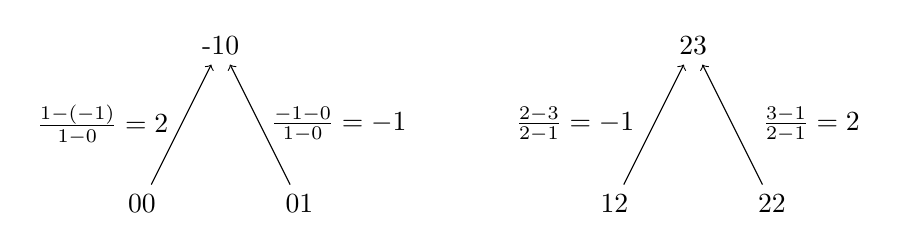
\begin{tikzpicture}
					\node (00) at (0, -1) {00};
					\node (-10) at (1, 1) {-10};
					\node (01) at (2, -1) {01};

					\draw[->] (00) -- node[xshift=-1cm]{$\frac{1 - (-1)}{1 - 0} = 2$}  (-10);
					\draw[->] (01) -- node[xshift=1cm]{$\frac{-1 - 0}{1 - 0} = -1$}  (-10);

					\node (12) at (6, -1) {12};
					\node (23) at (7, 1) {23};
					\node (22) at (8, -1) {22};

					\draw[->] (12) -- node[xshift=-1cm]{$\frac{2 - 3}{2 - 1} = -1$} (23);
					\draw[->] (22) -- node[xshift=1cm]{$\frac{3 - 1}{2 - 1} = 2$}(23);
				\end{tikzpicture}
				\caption{Piramidaal schema om de uniforme representatie te construeren.}
				\label{fig:open_uniform_naar_uniform}
			\end{figure}

			zodat $$P_{-10} = 2P_{00} - P_{01} = 2 * (2, 0, 2) - (1, 1, 1) = (3, -1, 3)$$ en $$P_{23} = -P_{12} + 2P_{22} = -(-1, 1, 1) + 2 * (-2, 0, 2) = (1, -1, -1) + (-4, 0, 4) = (-3, -1, 3)$$ Uiteindelijk kan men de coördinaten bekomen door elk coördinaat terug om te zetten naar hun twee-dimensionale representatie, zodat $P_{-10} = (1, -\frac{1}{3}), P_{01} = (1, 1), P_{12} = (-1, 1)$ en $P_{23} = (-1, -\frac{1}{3})$ de nieuwe controlepunten worden.

			\item De constructie is belangrijk omdat, indien deze transformatie niet toegepast wordt, het algoritme van Lane en Riesenfeld niet kan toegepast worden. Dit algoritme is namelijk in staat om zeer efficiënt en eenvoudig knopen toe te voegen aan de B-spline, zonder dat de vorm van de B-spline wijzigt.
		\end{itemize}
	}
\end{enumerate}

\section{NURBS constructie van cirkels en lijnsegmenten \accentuate{(§3.4.8 en slides)} }
\begin{enumerate}
	\vraag{Met welke \textit{NURBS} kun je exact een recht \textit{lijnsegment} door twee punten tekenen? Geef de precieze locatie van de \textit{controlepunten} (op een figuur), hun gewichten, en de corresponderende \textit{knopenvector}.}
	{
		\begin{itemize} 
			\item Figuur \ref{fig:vraag2_2_1} toont hoe een lijnsegment door twee punten getekend kan worden. Dit is de controleveelhoek die gebruikt wordt om onder andere elliptische en parabolische segmenten te produceren. Indien de gewichtsfactor $w$ gelijkgesteld wordt aan 0, krijgen we het lijnsegment $|P_0P_2|$. De knopenvector is $(0, 0 ; 0, 1 ; 1, 1)$.
			\begin{figure}[ht]
				\centering
				\includegraphics[width=0.5\textwidth]{vraag2_2_1}
				\caption{Recht lijnsegment door twee punten.}
				\label{fig:vraag2_2_1}
			\end{figure}
		\end{itemize}}
			
	\vraag{Met welke \textit{NURBS} bestaande uit \underline{één enkel segment} kun je een \textit{halve cirkel} (met centrum in de oorsprong en straal 1) tekenen? Geef de precieze locatie van de \textit{controlepunten} (op een figuur), hun gewichten, en de corresponderende knopenvector\textit{}. Wat is de graad van deze NURBS?}
	{
		\begin{itemize} 
		\item Figuur \ref{fig:vraag2_2_2} toont de toont de precieze locatie van de controlepunten. De knopenvector is $(0, 0, 0; 0 , 1; 1, 1, 1)$, de graad is 3 en de gewichten zijn $\{3, 1, 1, 3\}$.
		\begin{figure}[ht]
			\centering
			\includegraphics[width=0.5\textwidth]{vraag2_2_2}
			\caption{Een halve cirkel bestaande uit slechts één enkel segment met centrum in de oorsprong en straal 1.}
			\label{fig:vraag2_2_2}
		\end{figure}
		\end{itemize}
	}
			
	\vraag{Toon aan dat deze constructie inderdaad exact een halve cirkel oplevert.}{
		\begin{itemize} 
			\item Aangezien de cirkel een straal $R=1$ heeft, ziet de vergelijking van de cirkel er als volgt uit:
			$$\bigg(\frac{x}{w}\bigg)^2 + \bigg(\frac{y}{w}\bigg)^2 = 1$$
			Na omvorming rest ons enkel te bewijzen dat
			$$x^2 + y^2 - w^2 = 0$$ voor elk punt van de cirkel. Daarom stellen we het piramidaal schema op om een willekeurig punt $P_{tt}$ van het segment te berekenen. Figuur \ref{fig:vraag2_2_3} toont het schema dat gebruikt wordt. 			
			\begin{figure}[ht]
				\centering
				\includegraphics[width=0.5\textwidth]{vraag2_2_3}
				\caption{Piramidaal schema voor het bewijs van de halve cirkel.}
				\label{fig:vraag2_2_3}
			\end{figure}
			We weten dat 
			\begin{equation*}
				\begin{split}
					P_{000} & = (1, 0) \\
					P_{001} & = (1, 2) \\
					P_{011} & = (-1, 2) \\
					P_{111} & = (-1, 0) \\
				\end{split}
			\end{equation*}
			We kunnen deze punten echter voorstellen met homogene coördinaten, met $w$ het gewicht van dat punt:
			\begin{equation*}
				\begin{split}
					P_{000} & = (3,0, 3) \\
					P_{001} & = (1, 2, 1) \\
					P_{011} & = (-1, 2, 1) \\
					P_{111} & = (-3, 0, 3) \\
				\end{split}
			\end{equation*}
			Uitvoering van het piramidaal schema:
			\begin{equation*}
				\begin{split}
					P_{00t, x} & = 3 (1 - t) + 1  t = 3 - 2t \\
					P_{00t, y} & = 0  (1 - t) + 2  t = 2t \\
					P_{00t, w} & = 3  (1 - t) + 1  t = 3 - 2t\\
					P_{01t, x} & = 1  (1 - t) \;- \;1  t = 1 - 2t \\
					P_{01t, y} & = 2  (1 - t) + 2  t = 2 \\
					P_{01t, w} & = 1  (1 - t) + 1  t = 1 \\
					P_{11t, x} & = - 1  (1 - t) \;-\;3  t = -2t - 1 \\
					P_{11t, y} & = 2  (1 - t) + 0  t = 2 - 2t \\
					P_{11t, w} & = 1  (1 - t) + 3  t = 2t + 1 \\
				\end{split}
			\end{equation*}
			\begin{equation*}
				\begin{split}
					P_{0tt, x} & = (3-2t)(1 - t) + (1 - 2t)t = 3 - 4t \\
					P_{0tt, y} & = 2t(1 - t) + 2t = 4t - 2t^2 \\
					P_{0tt, w} & = (3 - 2t)(1 - t) + 1t = 3 - 4t +2t^2\\
					P_{1tt, x} & = (1 - 2t)(1 - t) + \;(-\;2t - 1)t = 1 - 4t \\
					P_{1tt, y} & = 2(1 - t) + (2 - 2t)t = 2 -2t^2 \\
					P_{1tt, w} & = 1(1 - t) + (2t + 1)t = 2t^2 + 1 \\
				\end{split}
			\end{equation*}

			Uiteindelijk kunnen deze laatste twee punten opnieuw geïnterpoleerd worden om het punt $P_{tt}$ te bekomen.
			\begin{equation*}
				\begin{split}
					P_{ttt, x} & = (3-4t)(1-t) + t(1-4t) = 3-6t \\
					P_{ttt, y} & = (4t-2t^2)(1-t)+ t(2-2t^2) = 6t-6t^2\\
					P_{ttt, w} & = (3-4t+2t^2)(1-t) + t(2t^2 + 1) = 3-6t+6t^2
				\end{split}
			\end{equation*}

			Nu dat we de $x$, $y$ en $w$ waarde van een punt kunnen bepalen voor eender welke waarde $t$, kan de cirkelvergelijking ingevuld worden: 
			\begin{equation*}
				\begin{split}
					|P_{tt, x}|^2 + |P_{tt, y}|^2 - |P_{tt, w}|^2 & = (3-6t)^2 + (6t-6t^2)^2 - (3-6t+6t^2)^2 \\
																  & = 9 - 36t + 36t^2 + 36t^2 - 72t^3 + 36t^4 - 36t^4 + 72t^3 - 72t^2 + 36t - 9 \\
																  & = 0
				\end{split}
			\end{equation*}
			De opgegeven figuur is dus een exacte halve cirkel.
		 \end{itemize}
		 }
			
	\vraag{Met welke \textit{NURBS} bestaande uit \underline{één enkel segment} kun je exact een \textit{volledige cirkel} (met centrum in de oorsprong en straal 1) tekenen? Geef de precieze locatie van de \textit{controlepunten} (op een figuur), hun gewichten, en de corresponderende \textit{knopenvector}. Wat is de graad van deze NURBS?}
	{
		\begin{itemize} 
			\item Maak gebruik van de gewichten $\{5, 1, 1, 1, 1, 5\}$ en knopenvector $\{0, 0, 0, 0, 0; 0, 1; 1,1,1,1,1\}$.  Figuur \ref{fig:vraag2_2_4} illustreert de precieze locatie van de controlepunten. De graad van deze NURBS is 5.  Punten $P_{00000}$ en $P_{11111}$ krijgen gewicht 5, de overige punten krijgen gewicht 1.
			\begin{figure}[ht]
				\centering
				\includegraphics[width=0.7\textwidth]{vraag2_2_4}
				\caption{Een volledige cirkel met slechts één segment van orde zes.}
				\label{fig:vraag2_2_4} 
			\end{figure}
		\end{itemize}}
\end{enumerate}

\section{Reflectiemodellen \accentuate{(§5.2, behalve §5.2.1.2 en §5.2.1.3) }}
\begin{enumerate}
	\vraag{Waarom zijn reflectiemodellen noodzakelijk?}{
		\begin{itemize} 
			\item De precieze fracties geabsorbeerd, doorgelaten, diffuus teruggekaatst en spiegelend teruggekaatst licht hangen af van zeer veel factoren: ondermeer de invalshoek, kleur en intensiteit van het invallend lichtstraal, de gladheid van het oppervlak, en de samenstelling, temperatuur, kleur en transparantie van het object spelen een belangrijke rol. Deze fysische verschijnselen moeten benaderd worden door een mathematisch model, wat men het reflectiemodel noemt. Hoe meer gesofisticeerd dit reflectiemodel is, hoe realistischer de uiteindelijk weergegeven figuur er zal uitzien, maar ook hoe complexer en langduriger de vereiste berekeningen zijn.
		\end{itemize}
		}
			
	\vraag{Omschrijf het lokale reflectiemodel (Phong-model). Geef ondermeer de berekenings-voorschriften, de betekenis van de parameters, en de nadelen.}{
		\begin{itemize} 
			\item Een lokaal reflectiemodel houdt enkel rekening met de interactie tussen een aantal puntvormige lichtbronnen, het reflecterend oppervlak en het oogpunt. Met licht dat teruggekaatst of gebroken wordt door andere objecten wordt geen rekening gehouden. In het Phong-model berekent men voor elke RGB-component de intensiteit, uitgestuurd in de richting $V$ van het oogpunt, als een som van drie bijdragen:
			\begin{equation*}
				\begin{split}
					I_{V, \hbox{rood}} & = I_{D, \hbox{rood}} + I_{S, \hbox{rood}} + I_{G, \hbox{rood}} \\ 
					I_{V, \hbox{groen}} & = I_{D, \hbox{groen}} + I_{S, \hbox{groen}} + I_{G, \hbox{groen}} \\ 
					I_{V, \hbox{blauw}} & = I_{D, \hbox{blauw}} + I_{S, \hbox{blauw}} + I_{G, \hbox{blauw}} \\ 
				\end{split}
			\end{equation*}
			\begin{itemize}
				\item \textbf{$I_D$} = Diffuse intensiteit.
				
					Deze bijdrage veronderstelt een ideaal mat oppervlak, en is bijgevolg enkel afhankelijk van de invallende lichtintensiteit $I_L$, de afstand $R$ van het oogpunt tot het oppervlak, en de hoek $\theta$ tussen de invallende lichtstraal $L$ en de normaal $N$ op het oppervlak.

					$$I_D = k_D\sum_L I_L \frac{\cos \theta}{R^2} \qquad 0 \leq k_D \leq 1$$

				\item \textbf{$I_S$} = Spiegelende intensiteit.

					Deze is het grootst in de richting $R$, die de teruggekaatste lichtstraal in de veronderstelling van een perfect reflecterend oppverlak weergeeft. Meestal neemt men een heuristische formule die dit gedrag vertoont, zoals,
					$$I_S = k_S\sum_L I_L \frac{\cos^n \Omega}{R^2} \qquad 0 \leq k_S \leq 1$$ 
					waarbij $n$ het getal is dat de gladheid van het oppervlak karakteriseert en $\Omega$ de hoek tussen $R$ en $V$.

				\item \textbf{$I_G$} = Intensiteit ten gevolge van omgevingslicht. 
				
				Dit wordt berekend als $$I_G = k_O \cdot I_O  \qquad 0 \leq k_O \leq 1$$ waarbij $I_O$ een constante van de volledige figuur is, en $k_O$ een materiaal afhankelijke coëfficiënt voorstelt.
				


			\end{itemize}
			Vooral ten gevolge van de triviale benadering voor het omgevingslicht zijn lokale reflectiemodellen niet in staat om schaduwen weer te geven, en zien alle objecten er eerder als plastiek uit.
		\end{itemize}
		}
	
			 
	\vraag{Geef en omschrijf (in het bijzonder de nadelen) van de drie mogelijke benaderingen voor de berekening van de \textit{lichtintensiteit van zichtbare punten}, indien men het object beschrijft aan de hand van een verzameling \textit{vlakke veelhoeken}.}{
		\begin{itemize} 
		\item \textbf{Uniform model:} Voor elk oppervlak wordt zijn normaal berekend die de lichtintensiteit voor het hele oppervlak bepaald. Het nadeel aan deze methode is dat elk punt van het oppervlak dezelfde intensiteit krijgt, wat zorgt voor een niet realistische voorstelling aangezien de verschillende segmenten, hoe klein ook, duidelijk zichtbaar zijn. Om dit te verhelpen wordt er in elk hoekpunt van het object een normaal $N_A$ berekend, door de oppervlakte normalen van de aangrenzende segmenten uit te middelen.
		\item \textbf{Gouraud-model:} Op basis van de normalen $N_A$ wordt eerst de lichtintensiteiten $I_A$ berekent, van de hoekpunten van het object. Elk ander punt van een veelhoek van het object kan berekend worden door lineaire interpolatie ten opzichte van de lichtintensiteiten van de verschillende hoekpunten van de veelhoek. Een nadeel van deze methode is dat, als de normalen in de hoekpunten gelijk zouden zijn, maar het object toch kartelingen bevat, het object uniform gekleurd zou worden. Nog een tekortkoming is een gebrekkige weergave van spiegelende terugkaatsing. Het Gouraud-model is ook onderhevig aan het Mach-banden effect.
		\item \textbf{Phong-model:} Dit model interpoleert niet de hoekpunten zoals in het Gouraud-model, maar de normalen zelf. Pas hierna wordt de lichtintensiteit van elk punt berekend. Het model produceert normalen in een willekeurig punt van de benaderende veelhoek, die de normalen op het reële, gekromde vlak beter benaderen. Het Phong-model is wel wat rekenintensiever dan het Gouraud-model.
	\end{itemize}}
			
\end{enumerate}

\section{1D Wavelet transformaties}
\begin{enumerate}
	\vraag{Bespreek met behulp van \textit{Multi-Resolutie-Analyse} de algemene concepten van wavelet transformaties. \accentuate{(§3.5.2)}}{
		\begin{itemize} 
			\item De multi-resolutie-analyse begint vanuit een rij lineaire functieruimten $V^t$. Deze functieruimten hebben als restrictie dat ze onderling genest moeten zijn:
			$$V^0 \subset V^1 \subset V^2 \subset V^3 \subset ...$$
			Een willekeurige functie $f^t(x)$ in $V^t$ kan geschreven worden als een lineaire combinatie van de basisvectoren $\phi^t(x)$ van deze ruimte. Deze basisvectoren worden ook wel schaalfuncties genoemd. 
			$$f^t(x) = \sum_{i=0}^{m_t - 1} c_i^t \cdot \phi^t_i(x)$$
			Meestal groepeerd men deze schalingsfuncties in een rijmatrix:
			$$\Phi^t(x) = \big(\phi_0^t(x)\quad\phi_1^t\quad...\quad\phi_{m_t - 1}^t(x)\big)$$

			Elke functie $f^{t - 1}(x)$ kan ook geschreven worden als een lineaire combinatie van de basisvectoren van $V^t$. Aangezien Alle $V^t$ onderling genest zijn, maakt $\phi^{t-1}(x)$ ook deel uit van $V^t$, met als gevolg dat elke basisvector $\phi_i^{t-1}(x)$ kan geschreven worden als een lineaire combinatie van de basisvectoren van $V^t$. Hiervoor wordt er een reductiematrix $P^t$ gebruikt:
			$$\Phi^{t - 1}(x) = \Phi^{t} \cdot P^t$$
			De reductiematrix $P^t$ bevat als aantal rijen het aantal schalingsfuncties in de ruimte $V^t$, en als aantal kolommen het aantal schalingsfuncties in de ruimte $V^{t - 1}$.

			Er zijn diverse keuzen voor de basisvectoren van $V^t$ mogelijk: er kan gekozen worden om de schalingsfuncties van $V^{t - 1}$ aan te vullen met zogenaamde wavelets uit $W^{t - 1}$. De wavelets uit $W^t$ worden genoteerd als $\psi_i^t$, en worden ook in een rijmatrix gegroepeerd:
			$$\Psi^t(x) = \big(\psi_0^t(x)\quad\psi_1^t(x)\quad...\quad\psi^t_{n_t - 1}(x)\big)$$
			Deze wavelets moeten voldoen aan de volgende voorwaarde
			$$<\phi_i^t(x) | \psi_j^t(x)> \equiv \int \big(\phi_i^t(x) \cdot \psi_j^t(x)\big) dx = 0, \qquad i \neq j $$
			zodat de wavelets semi-orthogonaal zijn. De orthogonaliteit van wavelets vereist bovendien
			$$<\psi_i^t(x) | \psi_j^t(x)> \equiv \int \big(\psi_i^t(x) \cdot \psi_j^t(x)\big) dx = 0, \qquad i \neq j $$
			wat meestal niet voldaan is, maar wel voor Haar-wavelets. Aangezien nu de wavelets van $W^{t - 1}$ deel uitmaken van $V^t$, kan elke wavelet $\phi_i^{t - 1}$ geschreven worden als een lineaire combinatie van de schaalfunctiers van $V^t$. Hiervoor wordt er een reductiematrix $Q^t$ gebruikt: 
			$$\Psi^{t - 1} = \Phi^t(x) \cdot Q^t$$
			De reductiematrix $Q^t$ heeft als aantal rijen het aantal schalingsfuncties in de ruimte $V^t$ en als aantal kolommen het verschil van de aantallen schalingsfuncties in $V^t$ en $V^{t - 1}$. 

			Elke functie kan dus op diverse manieren gerepresenteerd worden. Als de combinatie $V^t = V^{t - 1} + W^{t - 1}$ gebruikt wordt, kan elke functie $f^{t + 1}(x)$ als volgt geschreven worden:
			$$f^{t+1}(x) = \sum_{i=0}^{m_t - 1} c_i^t \cdot \phi^t_i(x) + \sum_{i=0}^{n_t - 1} d_i^t \cdot \psi^t_i(x)$$
			De coëfficiënten $c_i^t$ en $d_i^t$ worden in een rijmatrix voorgesteld:
		$$C^t = \begin{pmatrix} c_0^t \\ c_1^t \\ ... \\ c^t_{m_t - 1}\end{pmatrix}\qquad D^t = \begin{pmatrix} d_0^t \\ d_1^t \\ ... \\ d^t_{n_t - 1}\end{pmatrix}$$
			Op deze manier kan elke functie $f^{t + 1}(x)$ nu geschreven worden als:
			$$f^{t + 1}(x) = \Phi^t(x) \cdot C^t + \Psi^t(x) \cdot D^t$$
			De coëfficiëntenrijen $C^{t - 1}$ en $D^{t - 1}$ zijn equivalent met $C^t$. Om $C^t$ te berekenen volstaat het om de alternatieve ontwikkeling in basisvectoren van een willekeurige functie te vergelijken:
			\begin{equation*}
				\begin{split}
					\Phi^t(x) \cdot C^t = f^t(x) & = \Phi^{t-1}(x) \cdot C^{t-1} + \Psi^{t-1}(x) \cdot D^{t-1} \\
												 & = \Phi^{t} \cdot P^t \cdot C^{t-1} + \Phi^{t} \cdot Q^t \cdot D^{t-1} \\
												 & = \Phi^{t} \cdot (P^t\cdot C^{t - 1} + Q^t \cdot D^{t - 1})
				\end{split}
			\end{equation*}
			Om andersom, $C^{t - 1}$ en $D^{t - 1}$ te bepalen uit $C^t$ introduceert men de analyse $A^t$ en $B^t$:
			$$C^{t - 1} = A^t\cdot C^t\qquad D^{t - 1} = B^t\cdot D^t$$
			Hieruit kan afgeleidt worden dat de analyse en synthese ($P^t$ en $Q^t$) filters elkaars geïnverteerden zijn.
			\begin{equation*}
				\begin{split}
					\Phi^t(x) \cdot C^t = f^t(x) & = \Phi^{t-1}(x) \cdot C^{t-1} + \Psi^{t-1}(x) \cdot D^{t-1} \\
												 & = \Phi^{t-1}(x) \cdot A^t \cdot C^t + \Psi^{t-1}(x) \cdot B^t \cdot C^t \\
												 & = \Phi^{t} \cdot P^t \cdot A^t \cdot C^t + \Phi^{t} \cdot Q^t \cdot B^t \cdot C^t \\
												 & = \Phi^{t} \cdot (P^t  | Q^t) \cdot \bigg(\frac{A^t}{B^t}\bigg) \cdot C^t				
				\end{split}
			\end{equation*}
			zodat
			$$\bigg(\frac{A^t}{B^t}\bigg) = (P^t  | Q^t)^{-1}$$

		\end{itemize}}
			
	\vraag{Vertaal deze algemene concepten in het bijzonder geval van de \textit{Haar-wavelet} transformatie. \accentuate{(§3.5.1 \& §3.5.2)}}
	{
		\begin{itemize}
			\item Elke niveau $t$ benadering door een Haar-wavelet levert stuksgewijs constante functies op, constant in elk van de $2^t$ deelintervallen van het interval $[0, 1[$. Als Haar-schalingsfuncties neemt men meestal:
		$$\phi_i^t(x) = \phi(2^tx - i)\quad,\quad\hbox{met}\quad \phi(x) = 
			\begin{cases}
				0 &, x < 0 \\
				1 &, 0 \leq x < 1 \\
				0 &, x \geq 1
			\end{cases}$$

		Voorbeelden van de $V^0, V^1, V^2$ en $V^3$ schalingsfuncties zijn te zien op figuur \ref{fig:haar_schalingsfuncties}.
		\begin{figure}[ht]
			\centering
			\includegraphics[width=0.5\textwidth]{haar_schalingsfuncties}
			\caption{De $V^0, V^1, V^2$ en $V^3$ Haar-schalingsfuncties.}
			\label{fig:haar_schalingsfuncties}
		\end{figure}
		De reductiematrix $P^t$ wordt dan gegeven door:
		$$
		P^t = 
		\begin{pmatrix}
			+1 & 0 & ... & 0 & 0 \\
			+1 & 0 & ... & 0 & 0 \\
			0 & +1 &  ... & 0 & 0 \\
			0 & +1 &  ... & 0 & 0 \\
			... & ... & ... & ... & ... \\
			... & ... & ... & ... & ... \\
		 	0 & 0 & ... & +1 & 0  \\
		 	0 & 0 & ... & +1 & 0  \\
		 	0 & 0 & ... & 0 & +1  \\
		 	0 & 0 & ... & 0 & +1  \\
		\end{pmatrix}
		$$
		De Haar-wavelets zijn de wavelets die corresponderen met de Haar-schalingsfuncties, kunnen eveneens beschreven worden door:
		$$\psi_i^t(x) = \psi(2^tx - i)\quad,\quad\hbox{met}\quad \psi(x) = \begin{cases}
			0 &, x < 0 \\
			+ 1 &, 0 \leq x < 1/2 \\
			-1 &, 1/2 \leq x < 1 \\
			0 &, x \geq 1
		\end{cases}$$
		Voorbeelden van de $W^0, W^1, W^2$ en $W^3$ Haar-wavelets zijn te zien op figuur \ref{fig:haar_waveletfuncties}.
		\begin{figure}[ht]
			\centering
			\includegraphics[width=0.5\textwidth]{haar_waveletfuncties}
			\caption{De $W^0, W^1, W^2$ en $W^3$ Haar-wavelets.}
			\label{fig:haar_waveletfuncties}
		\end{figure}
		De wavelet $\psi(x)$ is de moederwavelet van de Haar-wavelet transformatie. Alle Haar-wavelets worden van de moederwavelet afgeleid door schaaloperaties en translaties. De reductiematrix $Q^t$ van de Haar-wavelet transformatie wordt gegeven door de volgende eenvoudige matrix, bestaande uit $2^t$ rijen en $2^t - 1$ kolommen:
		$$
		Q^t =
		\begin{pmatrix}
			+1 & 0 & ... & 0 & 0 \\
			-1 & 0 & ... & 0 & 0 \\
			0 & +1 &  ... & 0 & 0 \\
			0 & -1 &  ... & 0 & 0 \\
			... & ... & ... & ... & ... \\
			... & ... & ... & ... & ... \\
		 	0 & 0 & ... & +1 & 0  \\
		 	0 & 0 & ... & -1 & 0  \\
		 	0 & 0 & ... & 0 & +1  \\
		 	0 & 0 & ... & 0 & -1  \\
		\end{pmatrix}
		$$

		Voor de analyse filters van de Haar-wavelet transformatie bekomt men bijvoorbeeld volgende matrices met $2^t - 1$  rijen en $2^t$ kolommen:
		$$
		A^t =
		\begin{pmatrix}
			+1&+1&0&0&...&...&0&0&0&0 \\
			0&0&+1&+1&...&...&0&0&0&0 \\
			...&...&...&...&...&...&...&...&...&...\\
			0&0&0&0&...&...&+1&+1&0&0\\
			0&0&0&0&...&...&0&0&+1&+1
		\end{pmatrix}
		$$
		$$
		B^t =
		\begin{pmatrix}
			+1&-1&0&0&...&...&0&0&0&0 \\
			0&0&+1&-1&...&...&0&0&0&0 \\
			...&...&...&...&...&...&...&...&...&...\\
			0&0&0&0&...&...&+1&-1&0&0\\
			0&0&0&0&...&...&0&0&+1&-1
		\end{pmatrix}
		$$


	\end{itemize}
	}
	
			
	\vraag{Bespreek de noodzaak van \textit{spline-wavelets} (1D). Wat is het verband tussen de \textit{Haar-wavelet} transformatie en de \textit{spline-wavelet} transformatie? Geef een overzicht van de relatieve voor- en nadelen. }
	{
		\begin{itemize} 
			\item De Haar-wavelets laten enkel stuksgewijs constante functies toe, en zijn door het ontbreken van continuïteit (zelfs geen $C^0$ continuïteit) te beperkt voor de meeste toepassingen in de computergrafiek, in het bijzonder de voorstelling van krommen en oppervlakken. Daarom zoekt men een betere techniek. Via de stelling van Curry en Schoenberg kan men aantonen dat elke B-spline die met een bepaalde knopenvector voorgesteld kan worden, ook kan voorgesteld worden door een willekeurig verfijnde knopenvector. Dit heeft als gevolg dat alle mengfuncties behorend bij een bepaalde knopenvector, ook kunnen beschouwd worden als een lineaire combinatie van mengfuncties van een willekeurige verfijning van deze knopenvector. We kunnen dan de B-spline mengfuncties, behorend bij een rij onderling geneste knopenvectoren van een zelfde orde $k$, beschouwen als schaalfuncties van diverse niveau's van een spline-wavelet transformatie. In de praktijk wordt dit enkel gebruikt in combinatie met een open-uniforme knopenvector waarbij bovendien het aantal segmenten een macht van $2$ is, $2^t$, met $t$ het niveau van de Multi-Resolutie-Analyse schalingsfunctie:
			$$(0, ...,0\;;\;0,1,2...,2^t-1,2^t\;;\;2^t,...,2^t)$$
			De virtuele knopen komen aan beide kanten $k$ maal voor. Als spline-schalingsfuncties $\Phi^{t, k}$ heeft men de verzameling van $2^t + k - 1$ (het aantal controlepunten, waarvan 2 datapunten) mengfuncties $N_i(x) \equiv b_i^{t, k}(x)$, zoals die afgeleid kunnen worden met behulp van het algoritme van Cox en de Boor.
			
			De Haar-wavelet transformatie is een specifieke vorm van de spline-wavelet transformatie met $k = 1$. 

			De relatieve voor- en nadelen zijn:
			\begin{table}[ht]
				\centering
				\begin{tabular}{| l | p{0.3\textwidth} | l | p{0.3\textwidth}|}
					 \hline
					 & Spline-wavelet transformatie & & Haar-wavelet transformatie \\
					 \hline
					 + & Automatisch $C^{k - 2}$ continu & - & Zelfs geen $C^0$ continuïteit. \\
					 \hline
					 + & Veel toepassingen in de computergrafiek & - & Beperkte toepassing in de computergrafiek.\\
					 \hline
					 - & Voor alle $k > 1$ blijkt het enkel mogelijk te zijn om een verzameling semi-orthogonale spline-wavelets te construeren. & + & Altijd orthogonale wavelets. \\
					 \hline
					 - & Als gevolg van de semi-orthogonale spline-wavelets voor $k > 1$, kan men de analyse filters $A^{t,k}$ en $B^{t,k}$ slechts bekomen na expliciete numerieke inversie van de matrices samengesteld door de synthese filters $P^{t, k}$ en $Q^{t, k}$. & + & Bij Haar-wavelets kunnen de analyse filters bekomen worden door de synthese filters te transponeren. \\
					\hline
				\end{tabular}
			\end{table}
		\end{itemize}
	}

			
	\vraag{Beschrijf van lage orde 1D \textit{open-uniforme} spline-wavelet transformaties de vorm van achtereenvolgens de \textit{schaalfuncties}, de \textit{wavelets} en de \textit{synthese filters}.}
	{
		\begin{itemize} 
			\item Figuur \ref{fig:spline_schaling_wavelet} illustreert de $\Phi^{3, k}$ spline-schalingsfuncties en $\Psi^{3, k}$ spline-wavelets voor  $1 \leq k \leq 4$.
			\begin{figure}[ht]
				\centering
				\includegraphics[width=\textwidth]{spline_schaling_en_wavelets}
				\caption{De $\Phi^{3, k}$ spline-schalingsfuncties en $\Psi^{3, k}$ spline-wavelets voor $1 \leq k \leq 4$.}
				\label{fig:spline_schaling_wavelet}
			\end{figure}
			De synthesefilters $P^{t, k}$ bestaan elk uit $2^t + k -1$ rijen en $2^{t - 1} + k - 1$ kolommen. De eerste $k-1$ en laatste $k-1$ kolommen hebben geen eenvoudige structuur. Het middendeel bevat voor elke kolom slechts $k + 1$ niet-nul elementen, die op een constante factor na, de binomiaalcoëfficiënten blijken te zijn. Deze niet-nul elementen wordne per opeenvolgende kolom telkens twee rijen naar onderen verschoven. De synthese filters $P^{3, k}$ voor $1 \leq k \leq 4$ worden hieronder in matrixvorm gegeven:
			$$
			P^{3, 1} = 
			\begin{pmatrix}
				1 &   &   &   \\
				1 &   &   &   \\
				  & 1 &   &   \\
				  & 1 &   &   \\
				  &   & 1 &   \\
				  &   & 1 &  \\
				  &   &   & 1 \\
				  &   &   & 1 \\
			\end{pmatrix}
			\qquad
			P^{3, 2} = \frac{1}{2}
			\begin{pmatrix}
				2 &   &   &   & \\
				1 & 1 &   &   & \\
				  & 2 &   &   & \\
				  & 1 & 1 &   & \\
				  &   & 2 &   & \\
				  &   & 1 & 1 & \\
				  &   &   & 2 & \\
				  &   &   & 1 & 1\\
				  &   &   &   & 2\\
			\end{pmatrix}
			$$
			$$
			P^{3, 3} = \frac{1}{4}
			\begin{pmatrix}
				4 &   &   &   &   &   \\ % 1
				2 & 2 &   &   &   &   \\ % 2
				  & 3 & 1 &   &   &   \\ % 3
				  & 1 & 3 &   &   &   \\ % 4
				  &   & 3 & 1 &   &   \\ % 5
				  &   & 1 & 3 &   &   \\ % 6
				  &   &   & 3 & 1 &   \\ % 7
				  &   &   & 1 & 3 &   \\ % 8
				  &   &   &   & 2 & 2 \\ % 9
				  &   &   &   &   & 4 \\ % 10
			\end{pmatrix}
			\qquad
			P^{3, 3} = \frac{1}{16}
			\begin{pmatrix}
				16 &    &    &    &    &    &     \\ % 1
				8  & 8  &    &    &    &    &     \\ % 2
				   & 12 & 4  &    &    &    &     \\ % 3
				   & 3  & 11 &  2 &    &    &     \\ % 4
				   &    & 8  &  8 &    &    &     \\ % 5
				   &    & 2  & 12 & 2  &    &     \\ % 6
				   &    &    & 8  & 8  &    &     \\ % 7
				   &    &    & 2  & 11 &  3 &     \\ % 8
				   &    &    &    & 4  & 12 &     \\ % 9
				   &    &    &    &    &  8 &  8  \\ % 10
				   &    &    &    &    &    & 16  \\ % 11
			\end{pmatrix}
			$$
			De synthesefilters $Q^{t,k}$ bestaan uit $2^t +k - 1$ rijen en $2^t$ kolommen, en opnieuw worden in het middendeel van de matrix de niet-nul elementen per opeenvolgende kolom telkens twee rijen naar onder verschoven. De niet-nul elementen zijn groter in aantal ($3k - 1$) en minder eenvoudig uit te drukken. 
		\end{itemize}
		}

\end{enumerate}

\section{2D Wavelet transformaties \accentuate{(§4.5.1)}}
\begin{enumerate}
	\vraag{Bespreek de alternatieve methodes om 2D \textit{schaalfuncties en wavelets} te construeren.}
	{
		\begin{itemize} 
			\item De 2D-schaalfuncties $\Phi^t(x, y)$ blijven beperkt tot producten van twee 1D-schaalfuncties die afhankelijk zijn van één enkele variabele. Deze vereenvoudiging maakt het mogelijk om corresponderende 2D-wavelets te construeren op basis van 1D-schaalfuncties en 1D-wavelets.
			\item De 2D-wavelets kunnen op twee manieren geconstrueerd worden:
			\begin{enumerate}
				\item De standaard constructie berekent 2D-wavelets in een ruimte $W^t$, van willekeurige orde $t$, door alle mogelijke tensorproducten te nemen van alle 1D-wavelets in de ruimtes $W^i$ van orde $i$, $0 \leq i \leq t$, aangevuld met de 1D-schaalfuncties van de functieruimte $V^0$.
		
				\item De niet-standaard constructie neemt een aantal tensorproducten van 1D-wavelets in de ruimtes $W^i$ van orde $i$, $0\leq i\leq t$, aangevuld met 1D-schaalfuncties in de ruimtes $V^i$ van orde $i$.
			\end{enumerate}
		\end{itemize}
	}
			
	\vraag{Beschrijf, aan de hand van \textit{contourplotjes}, en voor elk van deze alternatieve methodes, de resulterende \textit{2D Haar-schaalfuncties en Haar-wavelets} van het laagste en het op één na laagste niveau.}
	{\begin{itemize} 
		\item \textbf{Standaard constructie}:
		Men bekomt de standaard 2D-Haar wavelets in $W^0$ en $W^1$ door de tensorproducten te berekenen van de 1D-Haar-wavelets in $W^0$ en $W^1$, aangevuld met $\phi^0$. De plustekens en mintekens duiden telkens de gebieden aan waar de wavelet +1 en -1 bedraagt. In de andere gebieden is de wavelet nul. Dit is te zien op figuur \ref{fig:standaard_constructie}.
		\begin{figure}[ht]
			\centering
			\includegraphics[width=0.5\textwidth]{standaard_constructie}
			\caption{De standaard constructie met behulp van contourplotjes.}
			\label{fig:standaard_constructie}
		\end{figure}
		\item \textbf{Niet-standaard constructie}: Men bekomt de niet-standaard 2D-Haar wavelets in $W^1$ door tensorproducten te berekenen van de 1D-Haar wavelets in $W^0$ en $W^1$, aangevuld met 1D-Haar schaalfuncties in $V^0$ en $V^1$. Dit is te zien op figuur \ref{fig:nietstandaard_constructie}
		\begin{figure}[ht]
			\centering
			\includegraphics[width=0.5\textwidth]{nietstandaard_constructie}
			\caption{De niet-standaard constructie met behulp van contourplotjes.}
			\label{fig:nietstandaard_constructie}
		\end{figure}
	 \end{itemize}}
\end{enumerate}

\section{Toepassingen van wavelet transformaties }
\begin{enumerate}
	\vraag{Geef de meest relevante toepassingen in de computergrafiek van \textbf{1D} \textit{Haar-wavelet} en \textbf{1D} \textit{spline-wavelet} transformaties. \accentuate{(§3.5.4)}}{\begin{itemize} 
		\item \textbf{Beeldcompressie:} De Haar-wavelet is wel nuttig bij beeldcompressie. In deze toepassing beschouwt men een lineair beeld bestaande uit $2^t$ pixels als een functie in de ruimte $V^t$ van Haar-schaalfuncties. De grijswaarden of kleurwaarden van de pixels bepalen de coëfficiënten $C^t$. Wavelet beeldcompressie voert een totale decompositie uit van een oorspronkelijk beeld, in termen van wavelets van verschillende niveau's $i (i < t)$, met coëfficiënten $D^i$, en de laagste niveau schaalfunctie. Termen met kleine wavelet coëfficiënten worden niet opgeslagen.
		\item \textbf{Manipulatie van krommen en oppervlakken:} Een kromme wordt doorgaans beschreven als een gemiddelde van de coördinaten van controlepunten (of datapunten), gewogen met behulp van mengfuncties $B_i(x)$:
		$$P(x) = \sum_i B_i(x)\cdot P_i$$
		Beschouw nu de mengfuncties als de schaalfuncties $\Phi^j(x)$ van een ruimte $V^j$, $\Phi^j(x) \equiv \{B_i(x), \forall i\}$, en de coördinaten van de controlepunten als coëfficiënten $C^j$ waarmee deze schaalfuncties moeten vermenigvuldigd worden, $C^j \equiv \{P_i, \forall i\}$, dan kan men hierop het principe van een filterbank toepassen. Door het recursief toepassen van de analyse filters $A^t$ en $B^t$ van een wavelet transformatie, bekomt men zowel coëfficiënten $C^t$ van lagere niveau schaalfuncties $\Phi^t(x)$, als coëfficiënten $D^t$ waarmee de corresponderende wavelets $\Psi^t(x)$ moeten vermenigvuldigd worden.
		\item \textbf{Gladmaken van krommen:} Bij deze toepassing worden kwadratische en vooral kubieke spline-wavelets aangewezen. De spline-wavelet decompositie produceert zeer snel benaderende B-splines, bepaald door $2^t + k - 1$ controlepunten, met verschillende gehele niveau's $t$ van gladheid.
		\item \textbf{Reconstructie van 3D beelden:} Aan de hand van vlakke contourlijnen kunnen 3D beelden gereconstrueerd worden. Elke dwarse doorsnede bestaat meestal uit een kromme, bepaald door een groot aantal controlepunten. Het is de bedoeling elk controlepunt van een dwarse doorsnede te verbinden met telkens twee opeenvolgende controlepunten van de volgende dwarse doorsneden. Op deze manier ontstaat tenslotte een driedimensionaal net van onderling met driehoeken verbonden controlepunten, dat het weer te geven oppervlak beschrijft. De complexiteit van het probleem wordt staptsgewijs vereenvoudigd door eerst opeenvolgende dwarse doorsneden volledig met behulp van een lineaire splinewavelet transformatie te reduceren. In de benadering van laagste niveau is het verbinden van de corresponderende controlepunten veel meer triviaal. Vervolgens wordt het oorspronkelijk beeld stapsgewijs gereconstrueerd, waarbij in elke stap triangulaties tussen de nog niet verbonden controlepunten en opeenvolgende dwarse doorsneden toegevoegd worden.
	\end{itemize}}
			
	\vraag{	Geef de meest relevante toepassingen in de computergrafiek van \textbf{2D} \textit{Haar-wavelet} en \textbf{2D} \textit{spline-wavelet} transformaties. \accentuate{(§4.5.2)}}{\begin{itemize} 
		\item \textbf{Compressie en reconstructie:} Bij kleurbeelden wordt de compressie uitgevoerd op de diverse kleurcomponenten, onafhankelijk van elkaar. De kleinste afwijking tussen het oorspronkelijk beeld en het geconstrueerde beeld, kan bekomen worden door systematisch de wavelets met de kleinste coëfficiënten te verwaarlozen, ongeacht hun orde.
		\item \textbf{Indexering:} Eerst wordt het te indexeren beeld met een Haar-wavelet transformatie gereduceerd. Vervolgens weerhoudt men enkel de coëfficiënten, in absolute waarde groter dan een bepaalde drempelwaarde. Tenslotte houdt men enkel rekening met het teken van de coëfficiënten. Een opzoeking kan als input een schets bevatten van het oorspronkelijke beeld. Deze input ondergaat dezelfde methode als om het beeld te indexeren. Vervolgens wordt de signatuur vergeleken met de signaturen in de databank. Beelden met de meeste overeenkomst komen in aanmerking als resultaat van deze opzoeking.
		\item \textbf{Gladmaken van oppervlakken:} Net zoals 1D-wavelet transformaties worden 2D-wavelet transformaties ook aangewend voor het gladmaken van oppervlakken.
		\item \textbf{Globale impact:} Controlepunten van een Bézier of NURBS oppervlak manipuleren heeft slechts een lokale impact. Als op dit oppervlak een 2D-wavelet decompositie uitgevoerd wordt, dan hebben die wijzigingen meer globaal karakter, naarmate het niveau lager is waarop men de wijzigingen uitvoert.  
		\item \textbf{Comprimeren:} Het biedt een eenvoudige manier om complexe oppervlakken in gecomprimeerde vorm op te slaan. het kan bijvoorbeeld gebruikt worden bij het doorsturen van beelden met een hoge resolutie over een netwerk met een relatief kleine bandbreedte. De zogenaamde \textit{progressieve transmissie} voert een volledige reductie van het oorspronkelijk beeld uit. Vervolgens wordt eerst de laagste orde benadering doorgestuurd, en vervolgens de diverse wavelet coëfficiënten, in volgorde van stijgende resolutie. Van zodra de $V^0$ benadering is ontvangen, kan al een model afgebeeldt worden. Achtereenvolgens kan telkens een hogere benadering doorgestuurd worden.
	\end{itemize}}
\end{enumerate}
	